\documentclass[conference, 10pt]{IEEEtran}
\usepackage{graphicx}
\usepackage{enumerate}
\usepackage{xspace}
\newcommand*{\eg}{e.g.\@\xspace}
\newcommand*{\ie}{i.e.\@\xspace}

\makeatletter
\newcommand*{\etc}{%
    \@ifnextchar{.}%
        {etc}%
        {etc.\@\xspace}%
}
\makeatother

\begin{document}

\title{CS270 Course Project Proposal:\\
Quick Alignment Algorithm for Burst Photography}

\author{\IEEEauthorblockN{Rundong Li}
\IEEEauthorblockA{36273800\\
SIST, ShanghaiTech University}
}

\maketitle

\begin{abstract}
    Photography quality of cell phones has received lot of attention. 
    Limited by small radius lens and tiny COMS sensors, digital images captured by
    mobile phones are easily suffer from noise on low illuminated areas, and unable to capture
    dynamic range on strongly illuminated areas. One possible solution is taking a burst of frames with different
    exposure settings, then merging into single high quality image.
    This rises the challenge of effectively aligning different frames before or after a series
    of other sophisticated operations. 
    We try to address this challenge in this course project.
\end{abstract}

\section{Proposal}
Photography quality of modern mobile phones is constrained by physical limitations
of their camera modules. On the one hand, small radius lens and tiny CMOS cells
limit the number of photons each pixel can gather; on the other hand, CMOS cells with limited photodiode volumes
are easily saturated when exposed on strong illuminations.
As a common example, when taking backlighted photos, dark noises
and over-exposure saturations often occur in conjunction, making post processing more difficult.

Compromising between extending exposure to eliminate dark noise, and reducing exposure to keep strong illuminated
areas from saturation, is somehow inflexible in \emph{single} image.
One possible solution is taking a \emph{burst} of frames with different exposure settings, then merge them into
single high dynamic ranged photo. This method is usually called \emph{burst photography}, as illustrated in Figure \ref{img::intro}.

However, this raises following challenges for image alignment algorithms:
\begin{enumerate}
    \item Each frame may has different degree of mismatches to adjacent frames, \eg when taking photos for
    moving senses, frames with logger exposure time may be more ``blur'' than frames with shorter exposure time.
    Single alignment strategy may not be suitable for both blur and still parts;
    \item Mobile phones have limited computation budget, and camera applications require real-time interaction,
    alignment algorithms thus should be fast, efficient and robust;
    \item Aligning multiple frames may introduce artifacts like ``ghosting'' (same object occurs multiple times
    in final image, due to mis-alignment), excessive denoising (image details are erased due to averaging
    multiple images) or ``cartoony'' (dynamic ranges of specific regions are saturated due to accumulating
    multiple images, thus the color tone of these regions look like cartoon);
\end{enumerate}

\begin{figure}[t]
\centering
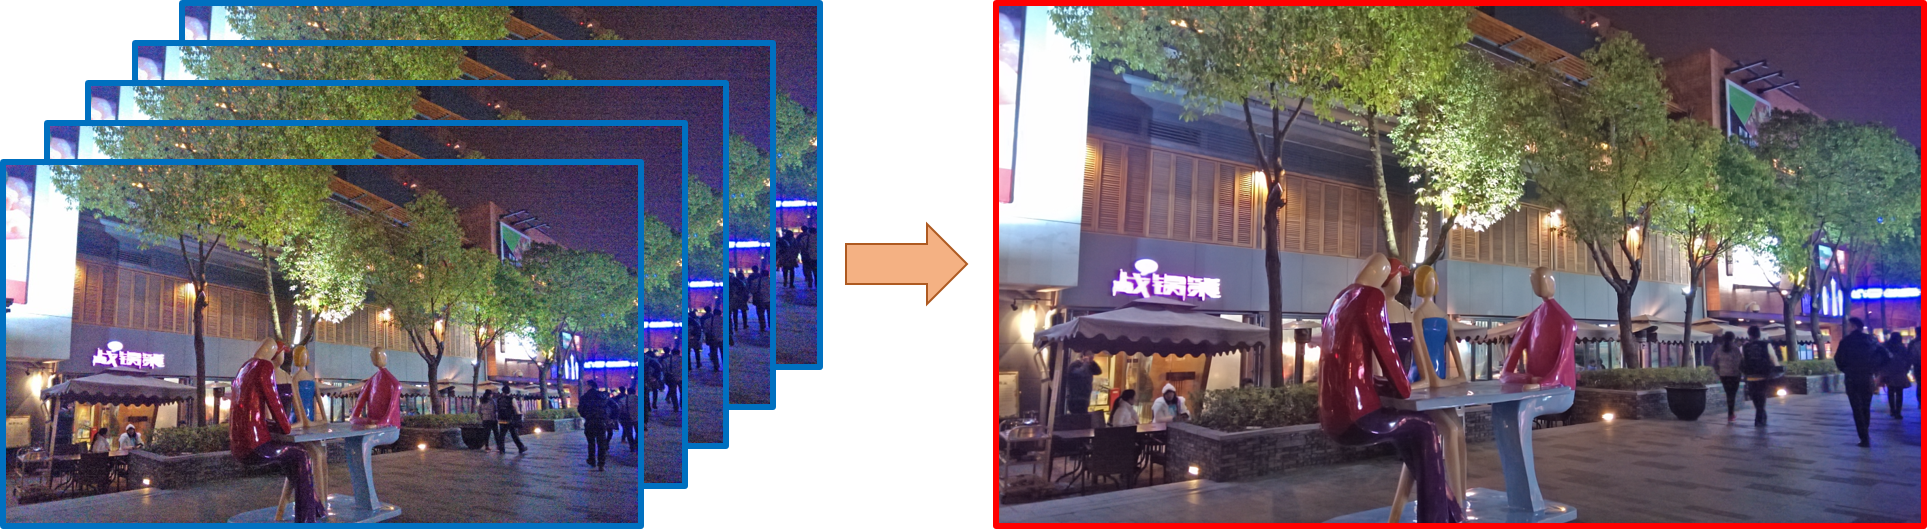
\includegraphics[width=\columnwidth]{img/intro_Liu_SIGGRAPH14.png}
\caption{A burst of frames can be align and merged into single high dynamic range photo.}
\label{img::intro}
\end{figure}

In this project, we try to address these challenges by a quick alignment algorithm. Possible techniques include:
\begin{enumerate}
    \item Performing coarse-to-fine alignment on Laplacian pyramid, the high-frequency components of input frames with different spatial sizes,
    to decrease computation coast;
    \item Using optical flow of input frames to assist alignment. Since computing optical flow is slow, accelerating
    techniques like optical flow network may be adopted;
    \item Using neural networks to extract feature maps with small spatial size, then apply alignment algorithms
    on these feature maps;
\end{enumerate}

Final results of this project will include an efficient alignment algorithm, along with a codebase to implement and benchmark
the proposed algorithm. This algorithm should be able to align 12-million-pixel resolution images with $\ge 5$ FPS on mobile phones with single CPU core.
Evaluation data set may be collected by taking target resolution photos by mobile phones, then apply stochastic jitter
to generate alignment bursts.

\end{document}
